\section{Density Plots}

 
Figure~\ref{lab:introplots122} shows the relationships between TCT and number of fish in each tank. Recall that for each sample replicate, there are eight technical replicates.


\begin{figure}[H]
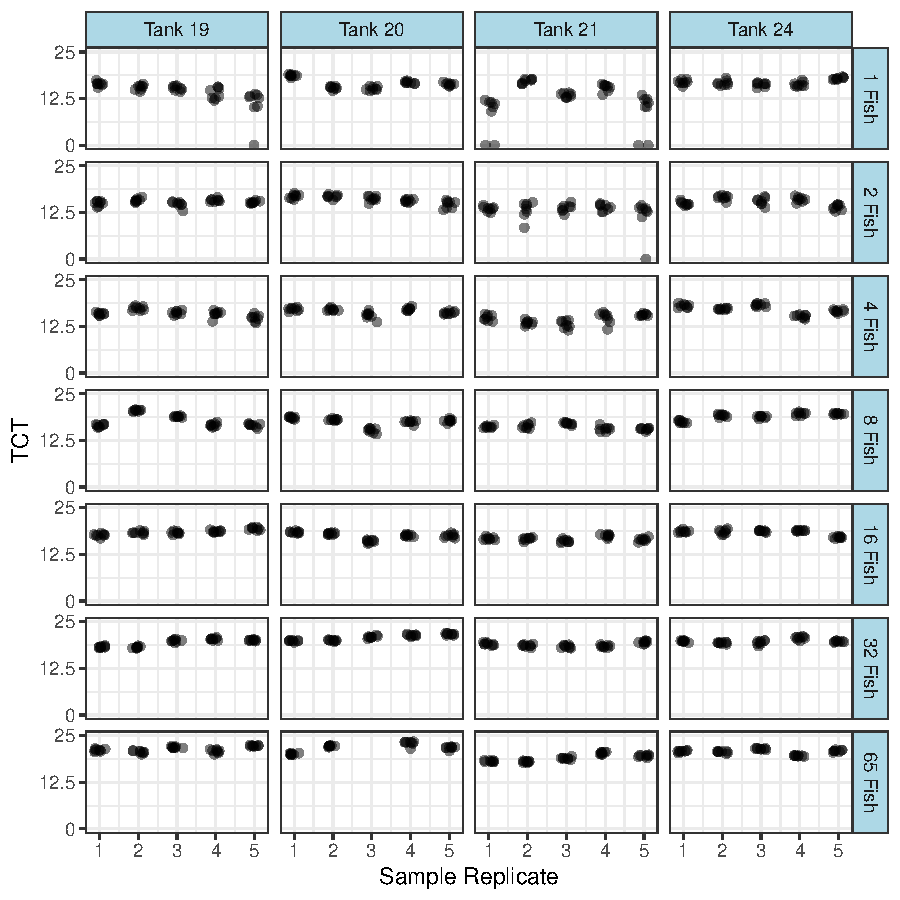
\includegraphics{Chapter3Images/gt.pdf}
\begin{center}
\caption{\hspace{1mm} Exploratory plots that plot the TCT for each number of fish in each tank. Each sample replicate has 8 technical replicates, each technical replicate has a TCT. }
\label{lab:introplots122}
\end{center}
\end{figure}








 In general, we notice TCT tends to increase as the number of fish increases. Although we have a relatively consistent increase in TCT as number of fish increases, there are several outliers. In particular, there are outliers for 1 Fish, Tank 19 and for 1 Fish, Tank 21. This may indicate that the presence of eDNA may not always be picked up in the lab. Although the sample had several technical replicates which did contain eDNA, some from the same sample replicate did not. As the density of fish increased, we see that we no longer have any major outliers, and the test for eDNA did not fail to pick up the presence of Coho eDNA.
  

\vspace{5mm}


Figure~\ref{lab:introplots1232} shows TCT values for the sample replicates taken for zero fish.  These are negative controls corresponding to sort codes 162-193 in Table 3.5. They were taken over a variety of tanks and days. The plots for tanks 1, 2, 3 and 4 correspond to the pilot experiment and give an idea of hatchery signal. The plots for tanks 19, 20, 21 and 24  are from `true' pre-fish negative controls for the density experiment.



\begin{figure}[H]
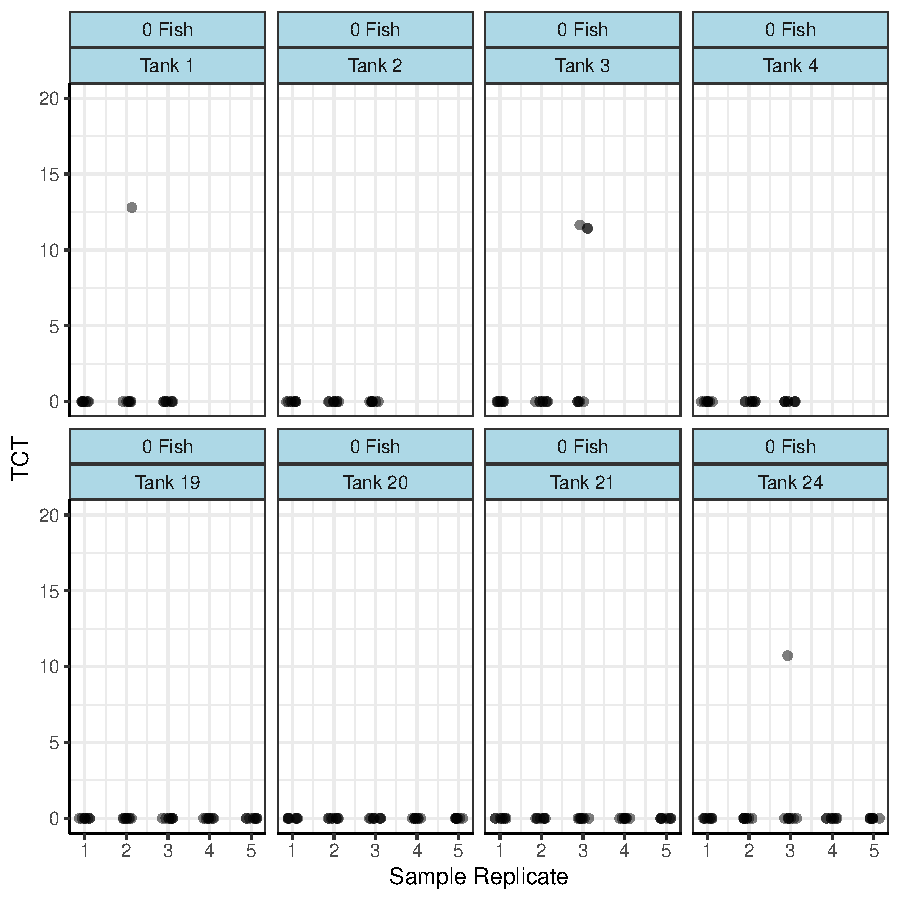
\includegraphics{Chapter3Images/gz2.pdf}
\begin{center}
\caption{\hspace{1mm} Plots of TCT for zero fish (Negative Controls). Notice there exists a slight Coho eDNA signal. This means that there could be Coho DNA present in the hatchery water. }
\label{lab:introplots1232}
\end{center}
\end{figure}




\begin{figure}[H]
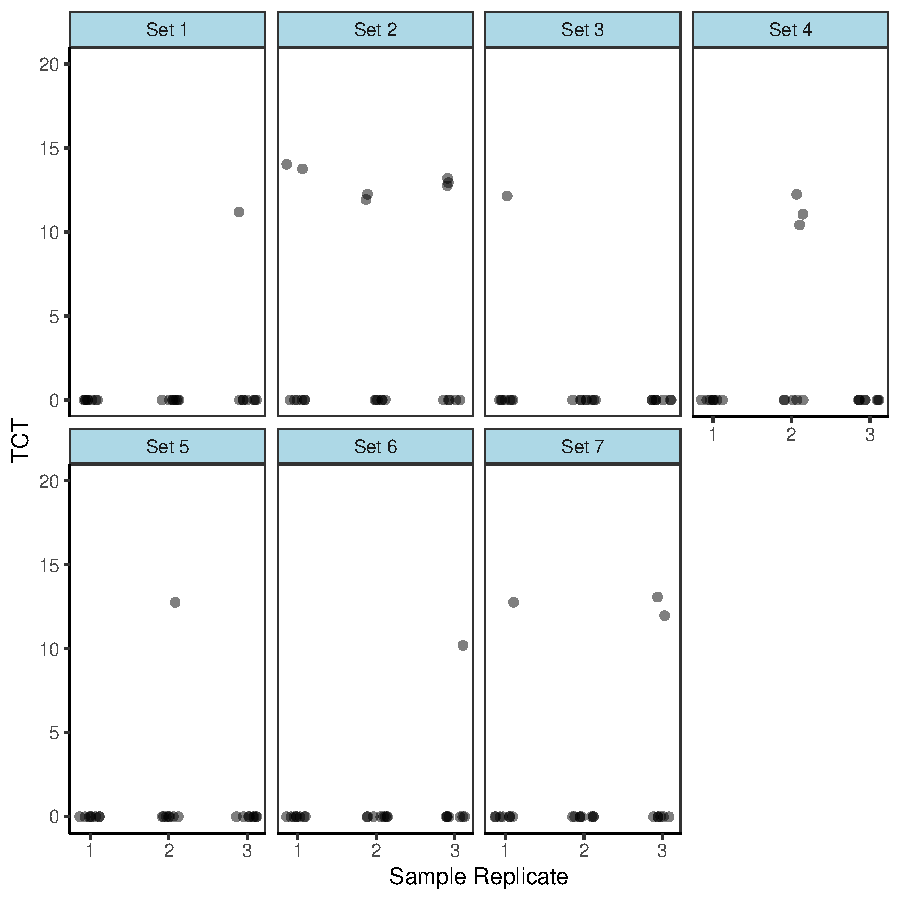
\includegraphics{Chapter3Images/gz3.pdf}
\begin{center}
\caption{\hspace{1mm}Additional plots of TCT for zero fish taken from tank 1. }
\label{lab:introplots123222}
\end{center}
\end{figure}





Figure~\ref{lab:introplots1232} and Figure~\ref{lab:introplots123222} are both plots of TCT values obtained from tanks in which no fish were present. Figure~\ref{lab:introplots1232} contains the negative controls for the main experiment, as well as TCT values obtained from the pilot experiment. Figure~\ref{lab:introplots123222} contains additional plots of TCT measurements taken from the pilot experiment. In general, the hatchery water appears to contain a small background signal of Coho. 